\chapter{Introduction to Deep Learning}
It seems logical to look at the brain's architecture for inspiration to build an intelligent machine. This is the logic that sparked artificial neural networks (ANN$_s$).
Machine learning models are inspired by the networks of biological neurons in our brains. ANN$_s$ are at the very core of deep learning. 
The first part of this chapter introduces artificial neural networks, starting with a quick visit to the very first ANN architectures and leading up to multilayer perceptrons, which are very used today. 

% Section 1 
\section{Logical Computations with Neurons}
The neurophysiologist Warren McCulloch and the mathematician Walter Pitts proposed, in 1943, a very simple model of the biological neuron, which became known as artificial neuron. It has one or more binary inputs and one binary output. The artificial neuron activates its output when more than a certain number of its inputs are active. 

Let's see what these networks do:
\begin{itemize}
    \item The network \ref{ANNs1} says: if neuron A is activated, then neuron C gets activated as well since it receives two input signals from neuron A. on the contrary if A is off, C is off as well.
    \item The network \ref{ANNs2} performs a logical \textit{AND}. Neuron C is activated only when both neurons A and B are activated. 
    \item The network \ref{ANNs3} performs a logical \textit{OR}. Neuron C gets activated if either neuron A or B is activated. Or both. 
    \item The network \ref{ANNs4} performs a complex logical proposition. Neuron C is activated only if neuron A is active and neuron B is off. They must follow this schema, otherwise, neuron C won't be activated. 
\end{itemize}

\begin{figure*}[t!]
    \centering
    \begin{subfigure}[b]{0.2\linewidth}
        \centering
        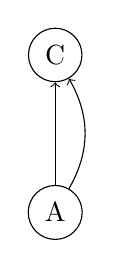
\begin{tikzpicture}[node distance=2cm]
                % First ANN
                \node[draw, circle] (A) at (0,0) {A};
                \node[draw, circle] (C) at (0,2) {C};
                
                \draw [->] (A) -- (C);
                \draw [->, bend right] (A) to (C);
            \end{tikzpicture}
            \caption{C=A}
            \label{ANNs1}
    \end{subfigure} \hfill
    \begin{subfigure}[b]{0.2\linewidth}
        \centering
       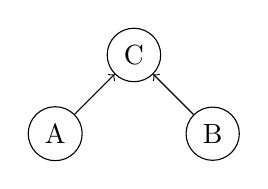
\begin{tikzpicture}[node distance=2cm]
            % Second ANN
            \node[draw, circle] (A) at (0, 0) {A}; 
            \node[draw, circle] (B) at (2, 0) {B}; 
            \node[draw, circle] (C) at (1, 1) {C}; 
            
            \draw [->] (A) -- (C);
            \draw [->] (B) -- (C);
        \end{tikzpicture}
        \caption{C = A $\land$ B}
        \label{ANNs2}
    \end{subfigure} \hfill
    \begin{subfigure}[b]{0.35\linewidth}
        \centering
        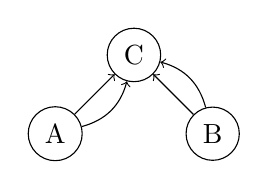
\begin{tikzpicture}[node distance=2cm]
            % Third ANN
            \node[draw, circle] (A) at (0, 0) {A};
            \node[draw, circle] (B) at (2, 0) {B};
            \node[draw, circle] (C) at (1, 1) {C};
            
            \draw [->] (A) -- (C);
            \draw [->, bend right] (A) to (C);
            \draw [->] (B) -- (C);
            \draw [->, bend right] (B) to (C);
        \end{tikzpicture}
        \caption{C = A $\lor$ B}
        \label{ANNs3}
    \end{subfigure} 
    \begin{subfigure}[b]{0.2\linewidth}
        \centering
        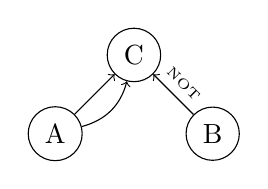
\begin{tikzpicture}[node distance=2cm]
            % Fourth ANN
            \node[draw, circle] (A) at (0, 0) {A};
            \node[draw, circle] (B) at (2, 0) {B};
            \node[draw, circle] (C) at (1, 1) {C};

            \draw [->] (A) -- (C);
            \draw [->, bend right] (A) to (C);
            \draw [->] (B) -- node[above, font=\tiny, sloped] {NOT} (C);
            
        \end{tikzpicture}
        \caption{C=A $\land \lnot$ B}
        \label{ANNs4}
    \end{subfigure}
    \caption{Artificial Neural Networks (ANNs) Performing Logical Computations - ANNs use multiple layers of neurons to perform logical computations.}
\end{figure*}


% Section 2
\section{The Perceptron}
The perceptron is one of the simplest ANN architectures. It is based on an artificial neuron called \textbf{threshold logic unit} (TLU), Figure \ref{fig:TLU Scheme}. The inputs and outputs are numbers, instead of binary on/off values, and each input connection is associated with a weight.  
The TLU computes a linear function of its inputs: 
\[
z = w_1 \cdot x_1 + w_2 \cdot x_2 + ... + w_n \cdot x_n + b = w^T \cdot x + b
\]
After that, it applies a step function to the result: 
\[
h_w(x) = f(z)
\]
The model parameters are the input weights \textbf{w} and the bias term \textit{b}.
A single TLU, can be used for simple linear binary classification. It computes a linear function of its inputs, and if the result exceeds a threshold, it outputs the positive class. Otherwise, it outputs the negative class. 

\begin{figure}[h!]
    \centering
    \begin{tikzpicture}[
        % define styles    
        init/.style={ 
             draw, 
             circle, 
             inner sep=2pt,
             font=\Huge,
             join = by -latex
        },
        squa/.style={ 
            font=\Large,
            join = by -latex
        }
    ]
        
        % Top chain x1 to w1
        \begin{scope}[start chain=1]
            \node[on chain=1] at (0,1.5cm)  (x1) {$x_1$};
            \node[on chain=1,join=by o-latex] (w1) {$w_1$};
        \end{scope}
        
        % Middle chain x2 to output
        \begin{scope}[start chain=2]
            \node[on chain=2] (x2) {$x_2$};
            \node[on chain=2,join=by o-latex] {$w_2$};
            \node[on chain=2,init] (sigma) {$\displaystyle\Sigma$};
            \node[on chain=2,squa,label=above:{\parbox{2cm}{\centering Activation\\ function}}]   {$f_{act}$};
            \node[on chain=2,squa,label=above:Output,join=by -latex] {$y_{out}$};
        \end{scope}
        
        % Bottom chain x3 to w3
        \begin{scope}[start chain=3]
            \node[on chain=3] at (0,-1.5cm) 
            (x3) {$x_3$};
            \node[on chain=3,label=below:Weights,join=by o-latex]
            (w3) {$w_3$};
        \end{scope}
        
        % Bias
        \node[label=above:\parbox{2cm}{\centering Bias \\ $b$}] at (sigma|-w1) (b) {};
        
        % Arrows joining w1, w3 and b to sigma
        \draw[-latex] (w1) -- (sigma);
        \draw[-latex] (w3) -- (sigma);
        \draw[o-latex] (b) -- (sigma);
        
        % left hand side brace
        \draw[decorate,decoration={brace,mirror}] (x1.north west) -- node[left=10pt] {Inputs} (x3.south west);
        
    \end{tikzpicture}
    
    \caption{The Threshold Logic Unit (TLU) - A fundamental building block of artificial neural networks, implementing a linear decision boundary to classify input data.}
    \label{fig:TLU Scheme}
\end{figure}

A perceptron is composed of one or more TLUs organized in a single layer, where every TLU is connected to every input. It is called \textit{fully connected layer}. The inputs constitute the \textit{input layer} and the final output is called \textit{output layer}.
It's possible to compute the outputs of a layer for more instance at once, just by applying the following formula:
\[
h_{W,b}(X) = \phi(XW + b)
\]

The parameters are: 
\begin{itemize}
    \item X represents the matrix of input features. 
    \item The weight matrix W contains all the connection weights. 
    \item The bias vector b contains all the bias terms (one per neuron).
    \item The function $\phi$ is called the \textit{activation function}. When the artificial neuron is a TLU, it is called a step function (the activation function will be discussed in the following chapter).
\end{itemize}

\subsection{How to train a perceptron}
Donald Hebb, considered the “father of neuropsychology”, in his 1949 book \textit{The Organization of Behavior}, suggested that when a biological neuron triggers another neuron often, the connection between these two neurons grows stronger. The connection weight between two neurons tends to increase when they fire simultaneously. This rule later became known as Hebb's rule. 
Perceptrons are trained using a variant of this rule that takes into account the error made by the network when it makes a prediction. The perceptron learning rule reinforces connections that help reduce the error. 
The rule is shown in the following equation:
\[
w_{i,j}^\text{next step} = w_{i,j} + \eta(y_i - \hat{y}_j) \cdot x_i
\]

where:
\begin{itemize}
    \item $w_{i,j}$ is the connection weight between the $i^\text{th}$ input and the $j^\text{th}$ neuron.
    \item $x_i$ is the $i^\text{th}$ input value of the current training instance. 
    \item $\hat{y}_j$ is the output of the $j^\text{th}$ output neuron for the current training instance. 
    \item $y_j$ is the target output of the $j^\text{th}$ output neuron for the current training instance. 
    \item $\eta$ is the learning rate. 
\end{itemize}

This perceptron training algorithm was proposed by Frank Rosenblatt who he got his inspiration from Hebb's rule. This algorithm is also called \textit{perceptron convergence theorem.}

% Section 3 
\section{Deep Neural Network}
A Multilayer Perceptron (MLP), Figure \ref{fig:MLP}, is composed of one input layer, one or more layers of TLUs \textit{hidden layers}, and one final layer of TLUs called the \textit{output layer}.
When an ANN contains a deep stack of hidden layers, it is called a \textit{deep neural network} (DNN). 
For many years researchers struggled to find a way to train MLPs. In the 1960s, some researchers discussed the possibility of using gradient descent to train neural networks but just in 1970, a researcher named Seppo Linnainmaa introduced a technique to compute all the gradients automatically and efficiently. This algorithm is called \textit{reverse-mode automatic differentiation}. 
In two passed through the network (one forward, one backward), it can compute the gradients of the neural network's error about every single model parameter.
It can find out how each connection weight and each bias should be tweaked to reduce the neural network's error. 
If you repeat this process of computing the gradients automatically and taking a gradient descent step, the neural network's error will gradually drop until it eventually reaches a minimum. This combination of reverse-mode automatic differentiation is called \textit{backpropagation}.
\tikzset{
    every neuron/.style={
    circle,
    draw,
    minimum size=1cm
  },
  neuron missing/.style={
    draw=none, 
    scale=4,
    text height=0.333cm,
    execute at begin node=\color{black}$\vdots$
  },
}

\begin{figure}[b!]
    \centering
    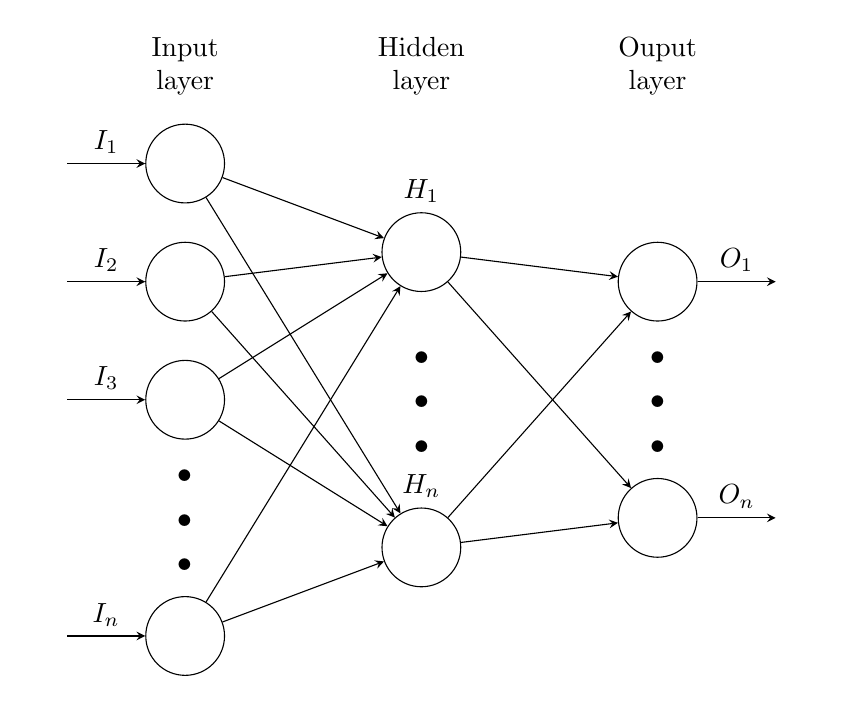
\begin{tikzpicture}[x=1.5cm, y=1.5cm, >=stealth]

    \foreach \m/\l [count=\y] in {1,2,3,missing,4}
      \node [every neuron/.try, neuron \m/.try] (input-\m) at (0,2.5-\y) {};
    
    \foreach \m [count=\y] in {1,missing,2}
      \node [every neuron/.try, neuron \m/.try ] (hidden-\m) at (2,2-\y*1.25) {};
    
    \foreach \m [count=\y] in {1,missing,2}
      \node [every neuron/.try, neuron \m/.try ] (output-\m) at (4,1.5-\y) {};
      
    \foreach \l [count=\i] in {1,2,3,n}
      \draw [<-] (input-\i) -- ++(-1,0)
        node [above, midway] {$I_\l$};
    
    \foreach \l [count=\i] in {1,n}
      \node [above] at (hidden-\i.north) {$H_\l$};
    
    \foreach \l [count=\i] in {1,n}
      \draw [->] (output-\i) -- ++(1,0)
        node [above, midway] {$O_\l$};
    
    \foreach \i in {1,...,4}
      \foreach \j in {1,...,2}
        \draw [->] (input-\i) -- (hidden-\j);
    
    \foreach \i in {1,...,2}
      \foreach \j in {1,...,2}
        \draw [->] (hidden-\i) -- (output-\j);
    
    \foreach \l [count=\x from 0] in {Input, Hidden, Ouput}
      \node [align=center, above] at (\x*2,2) {\l \\ layer};
    
    \end{tikzpicture}
    
    \caption{Architecture of a Multilayer Perceptron - A type of feedforward neural network that consists of multiple layers of interconnected neurons, with each neuron in one layer connected to every neuron in the next layer.}
    \label{fig:MLP}
\end{figure}

Backpropagation can be applied to all sorts of computational graphs, not just neural networks. In 1985, David Rumelhart, Geoffrey Hinton, and Ronald Williams published a paper \parencite{rumelhart1986learning} analyzing how backpropagation allowed neural networks to learn useful internal representations. Today, it is the most popular way to train neural nets.

\subsection{How does backpropagation work?}
It handles one mini-batch at a time, and it goes through the full training set multiple times. Each pass is called an \textit{epoch}. Each mini-batch enters the network through the input layer. The algorithm then computes the output of all the neurons in the first hidden layer, for every instance in the mini-batch. The result is passed on to the next layer, its output is computed and passed to the next layer, and so on until we get the output of the last layer, the output layer. 
This is the \textit{forward pass}.

The algorithm measures the network's output error. To calculate the error, it uses a loss function that compares the desired output and the actual output of the network and returns some measure of the error. 
Then, it computes how much each output bias and each connection to the output layer contributed to the error. The algorithm then measures how much of these error contribution came from each connection in the layer below, working backward until it reaches the input layer. 
Finally, the algorithm performs a gradient descent step to tweak all the connection weights in the network, using the error gradients just computed. 
It is important to initialize all the hidden layer's connection weights randomly, or else training will fail. If you initialize all weights and biases to zero, then all neurons in a given layer will be perfectly identical, and thus backpropagation will affect them in exactly same way, so they will remain identical. If instead, you randomly initialize the weights, you break the symmetry and allow backpropagation to train the neurons. 
Summing up, we can say that this technique makes predictions for a mini-batch, the forward pass, measures the error, then goes through each layer in reverse to measure the error contribution from each parameter, backward pass, and finally tweaks the weights and biases of the connections to reduce the error, gradient descent step. 



\subsection{The Vanishing/Exploding Gradients Problems}
The second stage of the backpropagation algorithm propagates the error gradient while moving from the output layer to the input layer. The algorithm uses these gradients to update each parameter with a gradient descent step after computing the gradient of the cost function for each network parameter. 
Unfortunately, when the algorithm descends to the lower layers, the gradient frequently gets smaller and smaller. As a result, training never converges to a good solution and the gradient descent update essentially leaves the connection weights of the lower layers unchanged. The vanishing gradient problem is what's happening here.
The inverse can also happen in some situations, causing the gradients to get larger until the layers receive massive weight updates and the algorithm diverges. This is the exploding gradients problem, which recurrent neural networks encounter most frequently. Deep neural networks more typically experience unstable gradients.

A paper \parencite{glorot2010understanding} by Xavier Glorot and Yoshua Bengio published in 2010 identified a few suspects, including the popular weight initialization technique and the combination of the sigmoid activation function. They demonstrated that the variation of each layer's outputs is significantly higher than the variance of its inputs when using this activation function and initialization technique. The activation function reaches saturation at the top layers as the network advances, with the variance increasing after each layer. The sigmoid function's mean is 0.5 rather than 0, which makes this saturation worse.
When inputs are high (positive or negative), as can be seen by looking at the sigmoid activation function, Figure \ref{fig:Activation Functions}, the function saturates at $0$ or $1$, with a derivative that is very close to $0$. As a result, when backpropagation begins, no gradient is left for it to propagate back through the network. 

Using weight initialization, where the weights are small random values, can help to prevent the exploding gradient problem. As presented in the paper, one popular initialization technique is called \textit{"Xavier"} or \textit{"Glorot"}, which adjusts the scale of the weights based on the number of input and output neurons in the layer. Another way to solve these problems is by using non-linear activation functions. Using non-linear activation functions such as ReLU, leaky ReLU, or Maxout instead of sigmoid or tanh can help mitigate the vanishing gradient problem (we are going to see activation functions in the following section).
The last two techniques we can use to avoid this problem are \textit{batch normalization} and \textit{regularization}, which will be shown in the following sections.

\subsection{Activation functions}
Rumelhart revised the structure of MLP to make backprop function properly: they replaced out the step function for the logistic function, better known as the \textit{sigmoid function}. This was crucial because there is no gradient to work with in the step function because the gradient descent cannot move on a flat surface, allowing it to advance somewhat at each step. The step function only contains flat segments. In actuality, aside from the sigmoid function, the backpropagation algorithm performs well with a wide variety of alternative activation functions. Here are two other popular choices. In the Figure \ref{fig:Activation Functions}, it's possible to see how they work.
\begin{itemize}
    \item \textit{The hyperbolic tangent function:} $tanh(z) = 2\sigma(2z) - 1$

    This activation function is S-shaped, continuous, and differentiable just like the sigmoid function, however its output value spans from -1 to 1, as opposed to 0 to 1, in the case of the sigmoid function. Because of this range, the output of each layer is more or less centered at zero at the start of training.

    \item \textit{The rectified linear unit function:} $ReLU(z) = max(0, z)$

    Although continuous, the ReLU function is unfortunately not differentiable at $z = 0$ and its derivative is $0$ for $z < 0$. But since it performs so well in practice and offers the benefit of being quick to compute, it has taken over as the standard. Since biological neurons appear to implement an activation function that is roughly sigmoid (S-shaped), researchers have focused on sigmoid functions for a very long time. ReLU, however, really performs better in ANNs in general. The biological analogy may have been misleading in this instance.
\end{itemize}
Why do we need activation functions? All you get when you combine many linear transformations is another linear transformation. Therefore, if there is no nonlinearity between the levels, even a deep stack of layers is equivalent to one layer, making it impossible to handle extremely complicated issues.
\begin{figure}
    \centering
    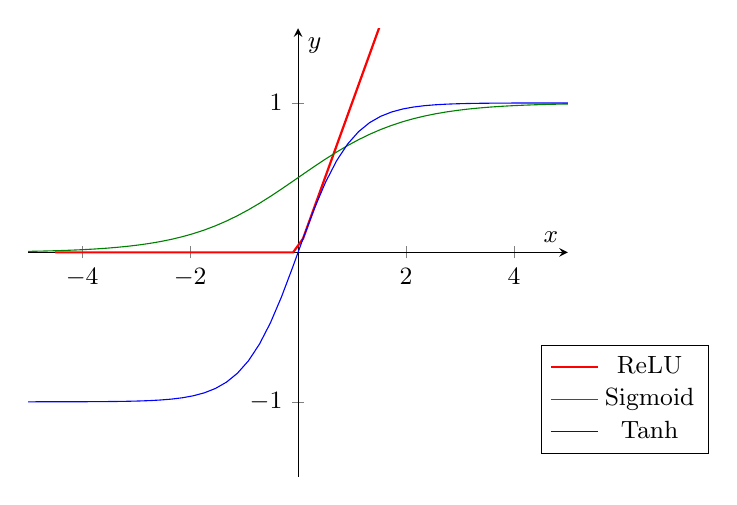
\begin{tikzpicture}
        \begin{axis}[
            axis lines = middle,
            xlabel = \(x\),
            ylabel = \(y\),
            xmin=-5.0,
            xmax=5.0,
            ymin=-1.5, 
            ymax=1.5,
            legend entries={ReLU,tanh,sigmoid},
            legend style={at={(0.95,0.05)},anchor=south west},
            %legend image post style={sharp plot,draw=red},
            cycle list name=color list,
            font=\small,
        ]
        % ReLU
        \addplot[color = red, thick, domain=-4.5:4.5, samples = 50] {max(0,x)};
        \addlegendentry{ReLU}
        % Sigmoid
        \addplot[color = green!50!black, samples=50] {1/(1+exp(-x))};
        \addlegendentry{Sigmoid}
    
        % tanh
        \addplot[color = blue, samples=50] {tanh(x)};
        \addlegendentry{Tanh}
        \end{axis}
    \end{tikzpicture}
    \caption{Activation Functions (ReLU, Sigmoid, Tanh) - Activation functions determine the output of a neuron in a neural network, and ReLU, Sigmoid, and Tanh are some commonly used activation functions that enable non-linear transformations of input data.}
    \label{fig:Activation Functions}
\end{figure}


\subsection{Hidden Layers}
Many issues can be solved by starting with a single hidden layer and producing acceptable results. Even the most complex functions can theoretically be modeled by an MLP with just one hidden layer. Deep networks, however, outperform shallow ones in terms of \textit{parameter efficiency} for complicated situations. Deep neural networks benefit from the fact that real-world data is frequently hierarchically structured as follows: The output layer and the highest hidden layers combine these intermediate structures to model high-level structures. Lower hidden layers model low-level structures, intermediate hidden layers combine these low-level structures to model intermediate-level structures, and the highest hidden layers model high-level structures like faces.

In conclusion, the neural network will function properly in many situations if you start with just one or two hidden layers. Increase the number of hidden layers for more complicated problems until the training set starts to become overfit. Large picture classification or speech recognition are two examples of extremely hard jobs that generally demand networks with dozens of layers and a huge amount of training data.

\subsection{Learning Rate and Optimizer}
There are more hyperparameters in an MLP than the number of neurons and hidden layers that can be changed. Some of the most important are listed below:
\paragraph{Learning rate} \mbox{} \\
\noindent The learning rate is the most important hyperparameter. The ideal learning rate is often equal to half the maximum learning rate.  Training the model for a few hundred iterations with a very low learning rate, like $10^{-5}$, and progressively raising it to a very high number, like $10$, is one method of determining a good learning rate. If you plot the loss as a function of the learning rate, you should notice that it first decreases.
However, after a while, the learning rate will become excessive, causing the loss to quickly increase again. The optimal learning rate will be slightly lower than the point at which the loss begins to increase.

\paragraph{Optimizer}\mbox{}\\
Equally important is selecting a better optimizer than just an odd mini-batch gradient descent. There are several optimizers that you can use to speed up the training but we are going to see just one, \textit{Adam}.
Adam -, which stands for \textit{adaptive moment estimation}, combines the concepts of momentum optimization and RMSProp: it tracks an exponentially decaying average of previous gradients, just like momentum optimization, and just like RMSProp, it tracks an exponentially decaying average of previously squared gradients. These are estimates of the gradients' mean and variance. The algorithm's name comes from the fact that the mean is sometimes referred to as the first instant and the variance as the second.
In other words, we can say the algorithm keeps track of two moving averages: the mean and the variance of the gradients; these moving averages are updated at each training step. This allows the algorithm to adapt to changes in the distribution of the gradients, which can be very beneficial for training deep neural networks:

\begin{equation}
    t = t + 1 
    \label{eq:1}
\end{equation}
\begin{equation}
    m_t = \beta_1 \cdot m_{t-1} + (1 - \beta_1) \cdot \nabla_{\theta} J(\theta) 
    \label{eq:2}
\end{equation}
\begin{equation}
    v_t = \beta_2 \cdot v_{t-1} + (1 - \beta_2) \cdot (\nabla_{\theta} J(\theta))^2 \label{eq:3}
\end{equation}
\begin{equation}
    \hat{m}_t = \frac{m_t}{1 - \beta_1^t}
    \label{eq:4}
\end{equation}
\begin{equation}
    \hat{v}_t = \frac{v_t}{1 - \beta_2^t}
    \label{eq:5}
\end{equation}
\begin{equation}
    \theta = \theta - \alpha \cdot \frac{\hat{m}_t}{\sqrt{\hat{v}_t} + \epsilon}
    \label{eq:6}
\end{equation}

where $\theta$ represents the parameters of the model, $\nabla_{\theta} J(\theta)$ is the gradient of the cost function J with respect to the parameters $\theta$, $\beta_1$ and $\beta_2$ are the decay rates of the moving averages, $\alpha$ is the learning rate, and $\epsilon is$ a small constant added to the denominator to prevent division by zero.

\hspace{1cm}

At each time step $t$, the mean $m_t$ and the variance $v_t$ of the gradients are updated using the equations \eqref{eq:2} and \eqref{eq:3}. Here, $m_{t-1}$ and $v_{t-1}$ represent the moving averages of the gradients and their squares from the previous time step. $\beta_1$ and $\ beta_2$ are hyperparameters that control the decay rate of the moving averages. They determine the amount of weight given to the past values of the gradients and their squares and the amount of weight given to the current gradient and its square.
After updating $m_t$ and $v_t$, the moving averages are corrected for bias using the equations \eqref{eq:4} and \eqref{eq:5}. The bias correction ensures that the moving averages are a better estimate of the true mean and variance of the gradients, especially at the start of the optimization process when $t$ is small.
Finally, the parameters $\theta$ are updated using the equation \eqref{eq:6}. Here, $\alpha$ is the learning rate, which determines the step size at which the parameters are updated. The term $\frac{\hat{m}_t}{\sqrt{\hat{v}_t} + \epsilon}$ is an approximation of the gradient of the cost function $J$ with respect to the parameters $\theta$. The addition of $\epsilon$ in the denominator is used to prevent division by zero.

This update rule balances the magnitude of the steps taken in the direction of the gradient with the magnitude of the gradient itself, allowing the optimization algorithm to make large steps in the directions with a high gradient and small steps in the directions with a low gradient. This makes the optimization process more efficient and helps the algorithm avoid getting stuck in local minima.
There are three variants of Adam: AdaMax, Nadam, and Adam W.

\subsection{Batch Normalization}
The danger of the vanishing/exploding gradients problems can be considerably reduced at the beginning of training by employing Glorot initialization in conjunction with ReLU, but this does not ensure that they won't reappear later on.
In a 2015 paper -, Sergey Ioffe and Christopher Szegedy suggested a method to solve these issues called \textit{batch normalization} (BN). The procedure includes inserting an operation into the model just before or after each hidden layer's activation function. The technique helps the model discover the ideal mean and scale for each input layer. In many circumstances, standardizing your training set is unnecessary if you include a BN layer as the initial layer of your neural network.

\hspace{1cm}

Let's say that we have a mini-batch of N examples, and the activations for a particular layer for one example is given by $X = [x_1, x_2, ..., x_d]$, where d is the number of neurons in the layer. The batch normalization algorithm consists of the following steps:

\begin{enumerate}
\item Calculate the mean and variance of the activations for the mini-batch:

\begin{equation}
\text{mean} = \frac{1}{N} \sum_{i=1}^{N} X_i
\end{equation}

\begin{equation}
\text{variance} = \frac{1}{N} \sum_{i=1}^{N} (X_i - \text{mean})^2
\end{equation}

\item Normalize the activations:

\begin{equation}
\hat{X} = \frac{X - \text{mean}}{\sqrt{\text{variance} + \epsilon}}
\end{equation}

where $\epsilon$ is a small constant added for numerical stability.

\item Scale and shift the normalized activations:

\begin{equation}
X_{\text{bn}} = \gamma \cdot \hat{X} + \beta
\end{equation}

where $\gamma$ and $\beta$ are learnable parameters.

\item Use the normalized and scaled activations as inputs to the next layer in the network.
\end{enumerate}

It is important to note that during training, the mean and variance of the activations are calculated on each mini-batch. During inference, the mean and variance are estimated using a running average that is updated during training. This allows the batch normalization layer to normalize the activations in a way that is consistent with the training data. In summary, the batch normalization algorithm normalizes the activations of a layer in a deep neural network by subtracting the mean and dividing by the standard deviation, scaling and shifting the result using learnable parameters, and using the normalized activations as inputs to the next layer in the network.

\hspace{1cm}

In conclusion, batch normalization is a widely used and effective technique for improving the training and performance of deep neural networks. It can help speed up training, prevent overfitting, and make the training process more robust to changes in the scale of the inputs and weights.

\subsection{Dropout}
Dropout, Figure \ref{fig:Dropout}, is one of the most popular regularization techniques for deep neural networks. It was proposed in a paper - by Geoffry Hinton et al. in 2012. 
It is a relatively straightforward algorithm: at each training step, each neuron (including input neurons but never output neurons) has a probability $p$ of being temporarily "dropped out," which means it will be completely ignored during this training phase but may be active during the next. This means that their activations are set to zero, and their incoming and outgoing connections are ignored. This has the effect of reducing the number of parameters in the network and making it more difficult for the network to memorize the training data. The dropout rate, also known as the hyperparameter p, is normally set between 10\% and 50\%; in recurrent neural networks, it is more likely to be between 20\% and 30\%. 

\begin{figure}[h!]
    \centering
    \begin{tikzpicture}[node/.style={circle, draw, thick}, scale = 0.85, transform shape]

      \foreach \y in {1,...,5}{
          \node[node] (i\y) at (0,\nodesep*\y) {};
          \node[node, right=\layersep of i\y] (h1\y) {};
          \node[node, right=\layersep of h1\y] (h2\y) {};
        }
    
      \node[node, right=\layersep of h22] (o1) {};
      \node[node, right=\layersep of h24] (o2) {};
    
      \foreach \source in {1,...,5}
      \foreach \dest in {1,...,5}{
          \path[-stealth, thick] (i\source) edge (h1\dest);
          \path[-stealth, thick] (h1\source) edge (h2\dest);
        }
      \foreach \source in {1,...,5}
      \foreach \dest in {1,2}
      \draw[-stealth, thick] (h2\source) -- (o\dest);
    
      \draw[-stealth, thick] (7.5,3*\nodesep) -- node[above,font=\Large\bfseries] {dropout} (9.5, 3*\nodesep);
    
      % Boundary
    
      \foreach \y in {1,...,5}
      \node[node, right=15em of h2\y] (di\y) {};
    
      \node[red,font=\huge] at (di1) {$\times$};
      \node[red,font=\huge] at (di3) {$\times$};
    
      \foreach \y in {1,...,5}
      \node[node, right=\layersep of di\y] (dh1\y) {};
    
      \node[red,font=\huge] at (dh11) {$\times$};
      \node[red,font=\huge] at (dh13) {$\times$};
      \node[red,font=\huge] at (dh14) {$\times$};
    
      \foreach \y in {1,...,5}
      \node[node, right=\layersep of dh1\y] (dh2\y) {};
    
      \node[red,font=\huge] at (dh22) {$\times$};
      \node[red,font=\huge] at (dh24) {$\times$};
    
      \node[node, right=\layersep of dh22] (do1) {};
      \node[node, right=\layersep of dh24] (do2) {};
    
      \foreach \source in {2,4,5}
      \foreach \dest in {2,5}
      \draw[-stealth, thick] (di\source) -- (dh1\dest);
    
      \foreach \source in {2,5}
      \foreach \dest in {1,3,5}
      \draw[-stealth, thick] (dh1\source) -- (dh2\dest);
    
      \foreach \source in {1,3,5}
      \foreach \dest in {1,2}
      \draw[-stealth, thick] (dh2\source) -- (do\dest);
    
    \end{tikzpicture}
    \caption{Dropout Scheme - A regularization technique used in neural networks to prevent overfitting by randomly dropping out some of the neurons in the network during training.}
    \label{fig:Dropout}
\end{figure}


For example, if the dropout rate is 0.5, then during each training iteration, on average, half of the units in the network will be dropped out. This results in a different, randomly perturbed network architecture at each training iteration, which helps prevent overfitting. The dropout rate can be tuned through experiments to find the optimal value for a given problem and network architecture. In general, a dropout rate of 0.5 is a good starting point, but the optimal value will depend on the specifics of the problem and the network architecture.

% Section 4
\section{Recurrent Neural Networks}
A class of nets called recurrent neural networks (RNNs) is capable of foreseeing the future. RNNs are capable of analyzing a variety of time series data, like the number of daily visitors to your website, the local hourly temperature, and more. An RNN can forecast the future using its knowledge of past patterns in the data, presuming of course that those patterns will continue to exist. Similar in appearance to a feedforward neural network, a recurrent neural network also includes connections pointing backward.

\hspace{1cm}

Let's discuss the simplest possible RNN, which consists of a single neuron taking inputs, producing output, and sending that output back to the neuron that received it, Figure \ref{fig:RNNs} (left). This recurrent neuron receives its own output from the previous time step $\hat{y}_{(t-1)}$ and the inputs $x_{(t)}$ at each time step $t$. At the first time step, the output is set at $0$, since there is no output at the previous time step. 
\begin{figure}
    \centering
    \begin{tikzpicture}[item/.style={circle,draw,thick,align=center}, itemc/.style={item,on chain,join}]
         \begin{scope}[start chain=going right,nodes=itemc,every join/.style={-latex,very thick},local bounding box=chain]
         \path node (A0) {$A$} node (A1) {$A$} node (A2) {$A$} node[xshift=2em] (At) {$A$};
         \end{scope}
         \node[left=1em of chain,scale=2] (eq) {$=$};
         \node[left=2em of eq,item] (AL) {$A$};
         \path (AL.west) ++ (-1em,2em) coordinate (aux);
         \draw[very thick,-latex,rounded corners] (AL.east) -| ++ (1em,2em) -- (aux) 
         |- (AL.west);
         \foreach \X in {0,1,2,t} 
         {\draw[very thick,-latex] (A\X.north) -- ++ (0,2em)
         node[above,item,fill=gray!10] (h\X) {$\hat{y}_{(\X)}$};
         \draw[very thick,latex-] (A\X.south) -- ++ (0,-2em)
         node[below,item,fill=gray!10] (x\X) {$x_\X$};}
         \draw[white,line width=0.8ex] (AL.north) -- ++ (0,1.9em);
         \draw[very thick,-latex] (AL.north) -- ++ (0,2em)
         node[above,item,fill=gray!10] {$\hat{h}_{(t)}$};
         \draw[very thick,latex-] (AL.south) -- ++ (0,-2em)
         node[below,item,fill=gray!10] {$x_t$};
         \path (x2) -- (xt) node[midway,scale=2,font=\bfseries] {\dots};
    \end{tikzpicture}
    \caption{A Recurrent Neuron (left) Unrolled through Time (right) - Recurrent neural networks (RNNs) are used to model sequences of data, with each neuron in the network receiving input not only from the current time step but also from the previous time step.}
    \label{fig:RNNs}
\end{figure}
This little network can be shown in relation to the time axis, Figure \ref{fig:RNNs} (right). "Unrolling the network through time" is what is meant by this. Each neuron receives the output vector from the previous time step, $\hat{y}_{(t-1)}$, as well as the input vector $x_{(t)}$, at each time step $t$. As you can see, now inputs and outputs are vectors. One set of weights is for the inputs $x_{(t)}$, and the other is for the outputs of the previous time step $\hat{y}_{(t-1)}$ for each recurrent neuron. These weight vectors will be abbreviated $w_x$ and $w_{\hat{y}}$. We can organize all the weight vectors into two weight matrices, $W_x$ and $W_{\hat{y}}$, if we think about the entire recurrent layer rather than just one recurrent neuron.
The output vector of the entire recurrent layer can then be calculated in a similar way to what one might anticipate.

\begin{equation}
\hat{y}_{(t)} = \sigma \left(W_{x}^{T} x_{(t)} + w_{\hat{y}}^{T} \hat{y}_{(t-1)} + b \right)
\end{equation}

Like feedforward neural networks, by putting all the inputs at time step t into an input matrix X, we can compute the output of a recurrent layer in one single step for an entire mini-batch.
    
\begin{equation}
    \begin{split}
    \hat{Y}_{(t)} & = \sigma \left(X_{(t)} W_x + \hat{Y}_{(t-1)} W_{\hat{y}} + b \right) \\
    & = \sigma \left(\begin{bmatrix} X_{(t)} & \hat{Y}_{(t-1)} \end{bmatrix} W + b \right) \text{with } W = \begin{bmatrix} 
    W_{x} \\
    W_{\hat{y}} 
    \end{bmatrix}
    \end{split}
    \label{eq:2_12}
\end{equation}

In above equation, \eqref{eq:2_12}, we can see:
\begin{itemize}
    \item $\hat{Y}_{(t)}$ is an \text{\textit{m} $\times$ $n_{\text{neurons}}$} matrix containing the layer's output at time step $t$ for each instance in the mini batch.
    \item $X_{(t)}$ is an \text{\textit{m} $\times$ $n_{\text{inputs}}$} matrix containing the inputs for all instances. 
    \item $W_{x}$ is an \text{$n_{\text{inputs}} \times n_{\text{neurons}}$} matrix containing the connection weights for the inputs of the current time step.
    \item $W_{\hat{y}}$ is an \text{$n_{\text{neurons}}$ $\times$ $n_{\text{neurons}}$} matrix containing the connection weights for the outputs of the previous time step.
    \item $b$ is a vector of size $n_{\text{neurons}}$ containing each neuron's bias term.
    \item The weight matrices $W_{x}$ and $W_{\hat{y}}$ are concatenated vertically into a single weight matrix $W$.
    \item The notation $\begin{bmatrix} X_{(t)} & \hat{Y}_{(t-1)} \end{bmatrix}$ represents the horizontal concatenation of the matrices $X_{(t)}$ and $\hat{Y}_{(t-1)}$.
\end{itemize}

Notice that $\hat{Y}_{(t)}$ is a function of $X_{(t)}$ and $\hat{Y}_{(t-1)}$, which is a function of $X_{(t-1)}$ and $\hat{Y}_{(t-2)}$, which is a function of $X_{(t-2)}$ and $\hat{Y}_{(t-3)}$, and so on. This makes $\hat{Y}_{(t)}$ a function of all the inputs since time $t = 0$ (that is $X_{(0)}, X_{(1)}, X_{(2)}, ...., X_{(t)}$). At the first time step, $t = 0$, there are no previous outputs, so they are assumed to be all zeros.

\subsection{How to train RNNs}
You could say that a recurrent neuron has a form of memory because its output at a given time step $t$ is a function of all its inputs from earlier time steps. A \textit{memory cell} is a component of a neural network that keeps a certain state over successive time steps.
The state of a cell at time step $t$, represented by the symbol $h_{(t)}$, is a function of some inputs at that time step and its state at the previous time step.
So, we can say $h_{(t)} = f\left(x_{(t)}, h_{(t-1)}\right)$. The previous state and the current inputs are functions of the output at time step $t$, indicated as $\hat{y}_{(t)}$.

\hspace{1cm}

An RNN can accept a series of inputs and generate different sequences:
\begin{itemize}
    \item \textit{Sequence-to-sequence network:} it takes a sequence of inputs and produces a sequence of outputs at each time step $t$.
    \item \textit{Sequence-to-vector network:} it takes a sequence of inputs, and you can consider only some outputs. For example, if you have 5 inputs, you might want only the last output, so you can ignore all the previous outputs.
    \item \textit{Vector-to-sequence network:} The input sequence is a vector that you pass into the network at each time step and let it output a sequence. 
    \item \textit{Encoder-decoder network:} This network is mostly used for translations. You pass a sentence in one language, and the output will be translated in another language. 
\end{itemize}

The idea is to unroll an RNN over time before using traditional backpropagation to train it. The term \textit{backpropagation over time} (BPTT) refers to this technique. The network is initially passed forward after it has been unrolled. After that, a loss function is used to evaluate the output sequence. 
\begin{equation}
    L(Y_{(0)}, Y_{(1)}, ...,Y_{(T)}; \hat{Y}_{(0)}, \hat{Y}_{(1)}, ...,\hat{Y}_{(T)})
\end{equation}

where $Y_{(i)}$ is the $i^{th}$ output, $\hat{Y}_{(i)}$ is the $i^{th}$ prediction and $T$ is the max time step. 
For example, if we think about \textit{sequence-to-vector network}, we want to compute only just the last two outputs of the network, ignoring the first three outputs. It means that the loss function isn't computed on all outputs, but just on the last two.

The unrolled network then propagates the gradients of that loss function backward. The gradients only pass through the outputs $\hat{Y}_{(3)}$ and $\hat{Y}_{(4)}$, since in the example the outputs $\hat{Y}_{(0)}$, $\hat{Y}_{(1)}$ and $\hat{Y}_{(2)}$ are not used to calculate the loss. Thusly, because $W$ and $b$ are identical parameters at every time step, their gradients will be changed numerous times during backprop. The parameters can be updated using a gradient descent step using BPTT when the backward phase is finished, and all the gradients have been computed.
This is how RNN training is made. 

\subsection{Long short-term memory (LSTM)}
In 1997, Seep Hochreiter and Jürgen Schmidhuber proposed the "Long Short-Term Memory" (LSTM) cell, which was progressively improved over time by other researchers \parencite{hochreiter1997long} . If the LSTM cell is viewed as a black box, it can be used in a similar way to that of a basic cell but will perform much better. Training will converge more quickly and find longer-term patterns in the data.

How do LSTM cells work? Figure \ref{fig:LSTM_cell} represents its architecture. The LSTM cell appears just like a standard cell from the outside, except for the fact that its state has been divided into two vectors, $h_{(t)}$ and $c_{(t)}$. The short-term state is represented by $h_{(t)}$, and the long-term state is represented by $c_{(t)}$.

The main concept is that the network can learn what to read from it, and what to discard or store in the long-term state. You can see that as the long-term state $c_{(t-1)}$ moves from left to right throughout the network, it first uses a forget gate to delete some memories before adding some new ones using an addition operation that includes memories that were chosen by an input gate. Without any further change, the result $c_{(t-1)}$ is sent out directly. Several memories are added, and some are deleted at each time step. The long-term state is copied and then passed via the tanh function following the addition operation. The output gate then filters the outcome. This produces the short-term state $h_{(t)}$.

\begin{figure}[b!]
    \centering
    \begin{tikzpicture}[
        % GLOBAL CFG
        font=\sf \scriptsize,
        >=LaTeX,
        % Styles
        cell/.style={% For the main box
            rectangle, 
            rounded corners=5mm, 
            draw,
            very thick,
            },
        operator/.style={%For operators like +  and  x
            circle,
            draw,
            inner sep=-0.5pt,
            minimum height =.2cm,
            },
        function/.style={%For functions
            ellipse,
            draw,
            inner sep=1pt
            },
        ct/.style={% For external inputs and outputs
            circle,
            draw,
            line width = .75pt,
            minimum width=1cm,
            inner sep=1pt,
            },
        gt/.style={% For internal inputs
            rectangle,
            draw,
            minimum width=4mm,
            minimum height=3mm,
            inner sep=1pt
            },
        mylabel/.style={% something new that I have learned
            font=\scriptsize\sffamily
            },
        ArrowC1/.style={% Arrows with rounded corners
            rounded corners=.25cm,
            thick,
            },
        ArrowC2/.style={% Arrows with big rounded corners
            rounded corners=.5cm,
            thick,
            },
        ]
    
    %Start drawing the thing...    
        % Draw the cell: 
        \node [cell, minimum height =4cm, minimum width=6cm] at (0,0){} ;
    
        % Draw inputs named ibox#
        \node [gt] (ibox1) at (-2,-0.75) {$\sigma$};
        \node [gt] (ibox2) at (-1.5,-0.75) {$\sigma$};
        \node [gt, minimum width=1cm] (ibox3) at (-0.5,-0.75) {Tanh};
        \node [gt] (ibox4) at (0.5,-0.75) {$\sigma$};
    
       % Draw opérators   named mux# , add# and func#
        \node [operator] (mux1) at (-2,1.5) {$\times$};
        \node [operator] (add1) at (-0.5,1.5) {+};
        \node [operator] (mux2) at (-0.5,0) {$\times$};
        \node [operator] (mux3) at (1.5,0) {$\times$};
        \node [function] (func1) at (1.5,0.75) {Tanh};
    
        % Draw External inputs? named as basis c,h,x
        \node[ct, label={[mylabel]Cell}] (c) at (-4,1.5) {\empt{c}{t-1}};
        \node[ct, label={[mylabel]Hidden}] (h) at (-4,-1.5) {\empt{h}{t-1}};
        \node[ct, label={[mylabel]left:Input}] (x) at (-2.5,-3) {\empt{x}{t}};
    
        % Draw External outputs? named as basis c2,h2,x2
        \node[ct, label={[mylabel]Label1}] (c2) at (4,1.5) {\empt{c}{t}};
        \node[ct, label={[mylabel]Label2}] (h2) at (4,-1.5) {\empt{h}{t}};
        \node[ct, label={[mylabel]left:Label3}] (x2) at (2.5,3) {\empt{\hat{y}}{t}};
    
    % Start connecting all.
        %Intersections and displacements are used. 
        % Drawing arrows    
        \draw [ArrowC1] (c) -- (mux1) -- (add1) -- (c2);
    
        % Inputs
        \draw [ArrowC2] (h) -| (ibox4);
        \draw [ArrowC1] (h -| ibox1)++(-0.5,0) -| (ibox1); 
        \draw [ArrowC1] (h -| ibox2)++(-0.5,0) -| (ibox2);
        \draw [ArrowC1] (h -| ibox3)++(-0.5,0) -| (ibox3);
        \draw [ArrowC1] (x) -- (x |- h)-| (ibox3);
    
        % Internal
        \draw [->, ArrowC2] (ibox1) -- (mux1);
        \draw [->, ArrowC2] (ibox2) |- (mux2);
        \draw [->, ArrowC2] (ibox3) -- (mux2);
        \draw [->, ArrowC2] (ibox4) |- (mux3);
        \draw [->, ArrowC2] (mux2) -- (add1);
        \draw [->, ArrowC1] (add1 -| func1)++(-0.5,0) -| (func1);
        \draw [->, ArrowC2] (func1) -- (mux3);
    
        %Outputs
        \draw [-, ArrowC2] (mux3) |- (h2);
        \draw (c2 -| x2) ++(0,-0.1) coordinate (i1);
        \draw [-, ArrowC2] (h2 -| x2)++(-0.5,0) -| (i1);
        \draw [-, ArrowC2] (i1)++(0,0.2) -- (x2);
    \end{tikzpicture}
    \caption{An LSTM Cell - A type of recurrent neural network cell that can selectively remember or forget information from previous time steps, making it particularly useful for processing sequential data such as text and speech.}
    \label{fig:LSTM_cell}
\end{figure}

Now let's see how gates perform. First, four separate fully connected layers take the current input vector $x_{(t)}$ and the previous short-term state $h_{(t-1)}$. Each one has a specific function:
\begin{itemize}
    \item The layer that outputs $g_{(t)}$ is the primary layer. Its regular functions include processing the inputs for the present $x_{(t)}$ and the past $h_{(t-1)}$ states. The output of this layer is not sent directly outside. Instead, its most fundamental parts are stored in the long-term state. The rest is dropped.
    \item Gate controllers are the three additional layers. The outputs are in the sigmoid activation function range, which is 0 to 1. The outputs from the gate controllers are fed into element-wise multiplication processes; if the output is a 0, the gate is closed; if a 1, the gate is opened. Particularly:
    \begin{itemize}
        \item The \textit{forget gate} $f_{(t)}$: determines which elements of the long-term state should be removed.
        \item The \textit{input gate} $i_{(t)}$: determines which $g_{(t)}$ components go into the long-term state.
        \item The \textit{output gate} $o_{(t)}$: determines which elements of the long-term state should be read and output at this time step, both to $h_{(t)}$ and $y_{(t)}$, 
    \end{itemize}
\end{itemize}

In conclusion, we can say that an LSTM cell can understand how to identify important input, \textit{"input gate"} role, and it can store in a long-term state, preserve and use it whenever it wants, \textit{"forget gate"} role.
There are more variants of the LSTM cell. Let's see now, the most used and important: the \textit{GRU} cell.

\begin{figure}[h!]
    \centering
    \begin{tikzpicture}[>=stealth, scale=1.25]
        %The rectangle :
        \filldraw[rounded corners, opacity=0.5, fill=white](0,0)rectangle(7,5);
        \draw[rounded corners, line width=0.4mm, tgray] (0,0)rectangle(7,5);
        %The connection lines and + x nodes : 
        \draw[thick, tgray, ->] (-1,4.5)node[left] {$h_{(t-1)}$}--(0,4.5);
        \draw[thick, tgray] (0,4.5)--(2,4.5);
        \draw[thick, tgray] (2.5,4.5)--(4.5,4.5);
        \draw[thick, tgray, ->] (5,4.5)--(8,4.5) node[right] {$h_{(t)}$};
        \draw[thick, tgray, ->] (6.5,4.5)--(6.5,6) node[right] {$y_{(t)}$};
        \node[tgray] (o1) at (2.25,4.5) {$\bigotimes$};
        \node[tgray] (o2) at (4.75,4.5) {$\bigoplus$};
        \draw[thick, tgray] (0.5,4.5)--(0.5,0.5);
        \draw[thick, tgray] (0.5,2)--(1,2); 
        \draw[thick, tgray] (1.5,2)--(2,2); 
        \draw[thick, tgray, ->] (1.25,1.35)--(1.25,1.8) node[midway, left] {$r_{(t)}$};
        \draw[thick, tgray, ->] (0.5,0.5)--(1.25,0.5)--(1.25,0.7);
        \draw[thick, tgray, ->] (2.25,1.35)  node[above left] {$z_{(t)}$} --(2.25,4.25);
        \draw[thick, tgray, ->] (2.25,-0.75) node[below] {$x_{(t)}$}--(2.25,0.7);
        \draw[thick, tgray, ->] (2.5,2)--(4.5,2)--(4.5,2.25);
        \draw[thick, tgray, ->] (1.25,0.5)--(2.25,0.7);
        \draw[thick, tgray, ->] (2.25,0.5)--(1.25,0.7);
        \node[tgray] (o3) at (1.25,2) {$\bigotimes$};
        \coordinate(o) at (3,3.5);
        \draw[tgray, thick] (2.25,3)--(o);
        \draw[tgray, thick, ->] (o)--(4.5,3.5);
        \filldraw[tgray] (o)circle(0.15) node[white, scale=0.5] {$1-$};
        \draw[thick, tgray, ->] (4.75,2.85)--(4.75,3.25);
        \draw[thick, tgray, ->]  (4.75,3.75)--(4.75,4.25);
        \node[tgray] at (4.75,3.5) {$\bigotimes$};
        %The small FC boxes
        %Box 1
        \draw[tgray] (1,0.75)rectangle(1.5,1.25); 
        \node[scale=0.85] at (1.25,1) {FC};
        \fill[tgray] (1,1.25)rectangle(1.5,1.3);
        %Box 2
        \draw[tgray] (2,0.75)rectangle(2.5,1.25); 
        \node[scale=0.85] at (2.25,1) {FC};
        \fill[tgray] (2,1.25)rectangle(2.5,1.3);
        %Box 3
        \draw[tgray] (4.25,2.3)rectangle(5.25,2.75);
        \node[scale=0.85] at (4.75,2.525) {FC};
        \fill[tgray] (4.25,2.75)rectangle(5.25,2.8);
    \end{tikzpicture}
    \caption{An GRU Cell - A type of recurrent neural network cell that uses gating mechanisms to control the flow of information through the cell, allowing it to selectively update or retain information from previous time steps.}
    \label{fig:my_label}
\end{figure}

\subsection{Gated Recurrent Unit (GRU)}
In a 2014 paper, Kyunghyun Cho et al. made the suggestion for the Gated Recurrent Unit (GRU) cell \parencite{cho2014learning}.
The GRU cell, which is an LSTM cell simplified, seems to work just as well. The main changes are as follows:

\begin{itemize}
    \item A single vector $h_{(t)}$ is created by combining the two state vectors.
    \item Both the input gate and the forget gate are managed by a single gate controller $z_{(t)}$. The input gate is closed $(1-1 = 0)$ and the forget gate is open $(= 1)$ if the gate controller sends a $1$. The opposite occurs if the output is a $0$. To put it another way, whenever a memory needs to be saved, the area where it will be stored must first be deleted.
    \item The entire state vector is output at each time step; there is no output gate. The main layer $g_{(t)}$ will only see certain portions of the prior state, thanks to a new gate controller $r_{(t)}$.
\end{itemize}

One of the key elements in the success of RNNs is the use of LSTM and GRU cells.



% Section 5 
\section{Convolutional Neural Networks}
A convolutional neural network (CNN) is a type of deep learning architecture commonly used in Computer Vision. 
CNN consists of multiple layers like the input layer, Convolutional layer, Pooling layer, and fully connected layers. 
The convolutional layer applies filter to the input imagine to extract features, the Pooling layer reduces the image in order to minimize computation,
and the fully connected layer makes the final prediction. The network learns the optimal filters through backpropagation and gradient descent. 

\subsection{Convolutional Layers}

%\usetikzlibrary{3d,decorations.text,shapes.arrows,positioning,fit,backgrounds}
\tikzset{pics/fake box/.style args={% #1=color, #2=x dimension, #3=y dimension, #4=z dimension
#1 with dimensions #2 and #3 and #4}{
code={
\draw[gray,ultra thin,fill=#1]  (0,0,0) coordinate(-front-bottom-left) to
++ (0,#3,0) coordinate(-front-top-right) --++
(#2,0,0) coordinate(-front-top-right) --++ (0,-#3,0) 
coordinate(-front-bottom-right) -- cycle;
\draw[gray,ultra thin,fill=#1] (0,#3,0)  --++ 
 (0,0,#4) coordinate(-back-top-left) --++ (#2,0,0) 
 coordinate(-back-top-right) --++ (0,0,-#4)  -- cycle;
\draw[gray,ultra thin,fill=#1!80!black] (#2,0,0) --++ (0,0,#4) coordinate(-back-bottom-right)
--++ (0,#3,0) --++ (0,0,-#4) -- cycle;
\path[gray,decorate,decoration={text effects along path,text={CONV}}] (#2/2,{2+(#3-2)/2},0) -- (#2/2,0,0);
}
}}
% from https://tex.stackexchange.com/a/52856/121799
\tikzset{circle dotted/.style={dash pattern=on .05mm off 2mm,
                                         line cap=round}}

\begin{tikzpicture}[x={(1,0)},y={(0,1)},z={({cos(60)},{sin(60)})},
font=\sffamily\small,scale=1.75]
%
% comment these out if you want to see where the axes point to
% \draw[-latex] (0,0,0) -- (3,0,0) node[below]{$x$};
% \draw[-latex] (0,0,0) -- (0,3,0) node[left]{$y$};
% \draw[-latex] (0,0,0) -- (0,0,3) node[below]{$z$};
% a plane
\foreach \X [count=\Y] in {1.6,1.4,1.2,1.2,1}
{
\draw pic (box1-\Y) at (\Y,-\X/2,0) {fake box=white!70!gray with dimensions 0.5 and {2*\X} and 1*\X};
}

\foreach \X/\Col in {6.5/red,6.7/green,6.9/blue}
{\draw[canvas is yz plane at x = \X, transform shape, draw = red, fill =
\Col!50!white, opacity = 0.5] (0,0.5) rectangle (2,-1.5);}
\draw[gray!60,thick] (6.3,-0.1,-1.6) coordinate (1-1) -- (6.3,-0.1,0.6) coordinate (1-2) -- (6.3,2.,0.6) coordinate (1-3) -- (6.3,2.1,-1.6) coordinate (1-4) -- cycle;
\draw[gray!60,thick] (7.1,-0.1,-1.6) coordinate (2-1) -- (7.1,-0.1,0.6) coordinate (2-2) -- (7.1,2.,0.6) coordinate (2-3) -- (7.1,2.1,-1.6) coordinate (2-4) -- cycle;
\foreach \X in {4,1,3}
{\draw[gray!60,thick] (1-\X) -- (2-\X);}
%
\node[draw,single arrow, orange,fill=orange!30] at (8,0.5,0) {GAP};
\node[circle,draw,blue,fill=blue!30] (A1) at (9,1,0) {~~~};
\node[circle,draw,red,fill=red!30,below=4pt of A1] (A2) {~~~};
\node[circle,draw,green,fill=green!30,below=18pt of A2] (A3) {~~~};
\draw[circle dotted, line width=2pt,shorten <=3pt] (A2) -- (A3);
\node[circle,draw,gray,fill=gray!20] (B1) at (10,1,0) {~~~};
\node[circle,draw,fill=gray!60,below=4pt of B1] (B2) {~~~};
\node[circle,draw,gray,fill=gray!20,below=18pt of B2] (B3) {~~~};
\draw[circle dotted, line width=2pt,shorten <=3pt] (B2) -- (B3);
\begin{scope}[on background layer]
\node[orange,thick,rounded corners,fill=orange!30,fit=(A1) (A3)]{};
\node[gray,thick,rounded corners,fill=gray!10,fit=(B1) (B3)]{};
\end{scope}
\foreach \X in {1,2,3}
{\draw[-latex] (A\X) -- (B2);}
\end{tikzpicture}